\scanpage{2}

\margin{(29.11.83)}

Soit $X$ surf. à bord compacte orientée, à structure torique
\inserted{(i.e. torseur sous $\mathbb U=\{z\in\mathbb C\mid |z|=1\}$\unsure{)}}
donnée sur les comp. connexes du bord.
On définit
\[
\begin{aligned}
\operatorname{SRT}(\unsure{\deleted{X}|X})={}&
\text{quotient du groupe des }\text{autom de }X
\text{ (}\text{\deleted{\unsure{en}} resp. }\text{l'orientation}\\
&\text{et les structures toriques) }\text{par la comp. neutre du}\\
&\text{sous-groupe }\operatorname{Aut}^!(\vec X)
\deleted{\unsure{\mathrm{bijec.}}}
\text{ de Aut }\text{qui induit}\\
&\text{l'identité sur }\partial X
\end{aligned}
\]

On a ainsi un dévissage de $\operatorname{SRT}(X)$ en trois étages
\[
\underbrace{S_{\unsure{*}}T^!(X)}_{
\operatorname{Aut}^!(\unsure{\vec X|\overline X})/\text{comp. neutre}}
\qquad\mathbb U^I\qquad\mathfrak S_I
\qquad I=\pi_0(\partial X)
\]
ou encore
\[
\mathbb Z^I\qquad T(X)\qquad\mathbb U^I\qquad\mathfrak S_I
\]

En fait, on définit can! un sous-groupe \inserted{droit}
$\mathbb R^I$ de $\operatorname{SRT}(X)$
contenant $\mathbb Z^I$, de telle façon qu'on ait
\[
\underbrace{\operatorname{SRT}^!(X)}_{
\substack{\text{noyau de}\\
\operatorname{SRT}^!(\alpha)\to\mathfrak S_I'}}
=\mathbb R^I.S_{\unsure{*}}T^!(X)
\]

\margin{\deleted{\unsure{et propre}}}
\diagram{
\begin{tikzcd}[column sep=small,row sep=small]
\mathbb R^I\arrow[dd,"\text{cocart}"{pos=.65,right}] &
\mathord{:}\arrow[l,phantom,"\unsure{\leftharpoonup}" description] &&\\
&&\unsure{\deleted{\lambda}|\lambda}&\\
\mathbb Z^I\arrow[r,hook]&
S_*T^!\arrow[uu,hook]\arrow[r,phantom,"\subset"]&
\operatorname{SRT}^!\arrow[r,phantom,"\subset"]&
\operatorname{SRT}
\end{tikzcd}
}

i.e. on a

\margin{\hfill$\unsure{*}$\par
\uline{NB} $\operatorname{SUT}(X)\simeq
T(X)\times_{\mathfrak S_I}\operatorname{Aut}((T_i)_{i\in I})$}

\margin{jusqu'ici on ne fait intervenir
que $S_*T^!(X)$; à l'exclusion de $S_*T(X)$,
dont la défini. exige une str. suppl.
$\uline{s}$, cf ci-dessous}

\diagram{
\begin{tikzcd}[column sep=small,row sep=large]
&\operatorname{SRT}(X)\arrow[d,no head,"\mathfrak S_I"]&\\
&\mathbb R^I.S_{\unsure{*}}T^!\arrow[dl,no head,"T^!"']
 \arrow[dr,no head,"\mathbb U^I"]&\\
\mathbb R^I\arrow[dr,no head,"\mathbb U^I"']&&S_*T^!(X)\\
&\mathbb Z^I\arrow[ur,no head,"T^!(X)"']&
\arrow[from=1-1,to=2-1,phantom,"\Bigg\{" description,"T(X)"']
\arrow[from=1-3,to=2-3,phantom,"\Bigg\}" description,"\operatorname{Aut}((T_i)_{i\in I})"]
\end{tikzcd}
}

d'où
\diagram{
\begin{tikzcd}[row sep=large,column sep=small]
\operatorname{SRT}\deleted{(X)}/\mathbb Z^I
 \overset{\text{déf}}=\operatorname{SUT}(X)
 \arrow[d,phantom,"\unsure{\downharpoonright|\downarrow}" description]&\\
T^!(X)\times\mathbb U^I&
\arrow[from=1-2,to=2-2,phantom,"\Bigg\}" description,"\mathfrak S_I"]
\end{tikzcd}
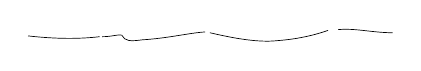
\begin{tikzpicture}[x=1cm,y=1cm]
\draw[line width=.25pt] (0,0) .. controls (.35,-.04) and (.66,-.04) .. (.91,-.01);
\draw[line width=.25pt] (.94,-.01) .. controls (1.07,-.01) and (1.13,.02) .. (1.19,.01)
 .. controls (1.23,-.07) and (1.3,-.07) .. (1.45,-.05)
 .. controls (1.78,-.03) and (2.06,.04) .. (2.25,.05);
\draw[line width=.25pt] (2.31,.04) .. controls (2.57,-.02) and (2.91,-.09) .. (3.17,-.06)
 .. controls (3.43,-.04) and (3.64,.01) .. (3.81,.07);
\draw[line width=.25pt] (3.94,.08) .. controls (4.16,.1) and (4.38,.04) .. (4.63,.04);
\end{tikzpicture}
}
\[
(*)\qquad1\longrightarrow\mathbb U^I\longrightarrow
\operatorname{SUT}(X)\longrightarrow\unsure{T}(X)-1
\]

De plus, chaque fois qu'on se donne un
marquage, i.e. un pt \deleted{\unsure{de}}
\[
\uline{s}=(s_i)\in
\prod_{i\in I=\pi_0(\partial X)}
\deleted{\unsure{(\mathbb U_i)}}T_i
\]
\margin{$T_i=$ comp. connexe (torique) de $\partial X$ d'indice $i$}

on trouve un plongement
\[
S_*T^{\deleted{\unsure{!}}}(X,\uline{s})\hookrightarrow\operatorname{SRT}(X)
\]
tel qu'on en déduise
\[
S_*T^{\deleted{\unsure{!}}}(X,\uline{s})
\mathbin{\wedge}_{\mathbb Z^I}\mathbb R^I
\simeq\operatorname{SRT}(X)
\]

\margin{1}
